\chapter{Building Your Network Marketing Business}

This chapter follows Jim Rohn's original third talk in the curated LazyingArt LLC sequence, written from the Video2Book transcript rather than from a classroom blackboard record. Because no validated mathematical screenshots survive for this lecture, the formulas and diagrams below are conservative editorial shorthand for repeated spoken comparisons and numerical examples. The lecture has a clear quantitative spine: profits over wages, part-time profit over wage dependence, response over circumstance, averages over emotional volatility, and service over self-enclosure.

\section{From Farm Labor to Philosophy}

Rohn opens autobiographically. He is the Idaho farm boy who knows how to milk cows, and not much else, and the point of the story is not nostalgia. The point is that a life may begin with very little formal leverage and still turn sharply once a new philosophy is acquired. Network marketing matters in this telling not merely because it offers a product, a compensation plan, or an entry point. It matters because it offers a framework for reading one's own life.

That is why he insists, very early, that technique by itself is not decisive. One may have the best product, the finest support, and every technique in the world, but if the philosophy is weak, the mechanism is inert. In these notes we should keep that ordering. The lecture does not begin with a method. It begins with a hidden variable.

He briefly returns to nutrition as an example of belief put into practice. That passage is not presented mathematically, but it serves an important structural role. It says that belief is not a mood; it is a principle of sustained action. What one studies, practices, and passes on becomes a life-forming discipline.

\subsection{Question \& Answer}

\paragraph{Question.} Why does the lecture treat philosophy, rather than product or technique, as the decisive cause?

\paragraph{Answer.} Because product and technique are presented as available inputs, while philosophy governs whether we persist, whether we interpret setbacks correctly, and whether we turn the available mechanism into actual results. In that sense philosophy is the control variable and the later techniques are downstream instruments.

\section{Profits, Wages, and the Magic of Part-Time}

The first major principle is stated as a slogan, but it is not left as a slogan. We may write, as a compact shorthand for the hierarchy he repeatedly asserts,
\begin{equation}
P > W.
\end{equation}
Here \(W\) denotes wages and \(P\) denotes profits. This is not Rohn's own notation, but it is faithful to the spoken contrast. Wages make a living; profits make a fortune. The lecture wants us to hear that as a structural distinction, not as a merely emotional preference:
\begin{equation}
W \longmapsto \text{a living},
\qquad
P \longmapsto \text{a fortune}.
\end{equation}

He then widens the contrast into a political-economic claim. Capital in the hands of the people generates ingenuity; capital concentrated in the state destroys it. His concrete numerical dramatization is the devastation of East Germany:
\begin{equation}
\$1\text{ trillion}
=
\$500\text{ billion already spent}
+
\$500\text{ billion still to go}.
\end{equation}
The number is doing rhetorical work. A bad philosophy is not merely wrong in theory. It becomes concrete damage.

But the lecture does not stay at the level of systems. Once profits have been distinguished from wages, the practical question is immediate: how does an ordinary person enter the field of profit? Rohn's answer is the magic of part-time. One does not begin by abandoning the wage job. One begins with a narrow, realistic time budget:
\begin{equation}
h_{\mathrm{pt}} \in \{10,12,15\}\ \text{hours per week}.
\end{equation}
From there the lecture builds two thresholds. The first threshold is equality:
\begin{equation}
P_{\mathrm{pt}} = W_{\mathrm{ft}}.
\end{equation}
The second threshold is dominance:
\begin{equation}
P_{\mathrm{pt}} = 2W_{\mathrm{ft}}.
\end{equation}
Again, the notation is editorial, but the sequence is transcript-faithful. Part-time profit first reaches the full-time wage, and then surpasses it by a factor of two. Only after this sequence is in place does he turn to recruiting logic.

\begin{figure}[h]
\centering
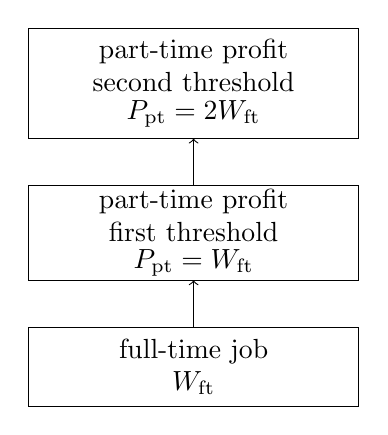
\begin{tikzpicture}[x=1cm,y=1cm]
\draw (0,0) rectangle (4.2,1.0);
\node at (2.1,0.5) {\shortstack{full-time job\\$W_{\mathrm{ft}}$}};

\draw (0,1.6) rectangle (4.2,2.8);
\node at (2.1,2.2) {\shortstack{part-time profit\\first threshold\\$P_{\mathrm{pt}}=W_{\mathrm{ft}}$}};

\draw (0,3.4) rectangle (4.2,4.8);
\node at (2.1,4.1) {\shortstack{part-time profit\\second threshold\\$P_{\mathrm{pt}}=2W_{\mathrm{ft}}$}};

\draw[->] (2.1,1.0) -- (2.1,1.6);
\draw[->] (2.1,2.8) -- (2.1,3.4);
\end{tikzpicture}
\end{figure}

The lecture's most practical observation in this section is that the same quantity of money has a different persuasive force depending on where it sits. An extra thousand dollars a month earned full-time is absorbed into maintenance. An extra thousand earned part-time is read as evidence of a new mechanism:
\begin{align}
\$1000/\text{month}_{\mathrm{ft}} &\Rightarrow \text{maintenance of an existing life},\\
\$1000/\text{month}_{\mathrm{pt}} &\Rightarrow \text{visible change in lifestyle}.
\end{align}
This is why part-time earnings generate an invitation. They alter the margin of life, and that alteration becomes legible to other people.

\subsection{Question \& Answer}

\paragraph{Question.} Why is part-time profit a stronger invitation than the same amount earned full-time?

\paragraph{Answer.} Because the lecture treats part-time money not as one more wage stream but as proof of a second economic mechanism. The same nominal sum carries more narrative force when it produces vacations, cars, clothes, or freedom without replacing the original job. What recruits is not only the amount; it is the altered structure of life.

\section{Wind, Sail, and the Logic of Self-Change}

The lecture now leaves the local arithmetic of part-time work and generalizes. It is not what happens that determines the future; it is what we do about what happens. To compress the analogy into a schematic we may write
\begin{equation}
O = f(E,S),
\end{equation}
where \(O\) is outcome, \(E\) is shared environment, and \(S\) is what the lecture calls the set of the sail. This is not formal economics. It is a compact rendering of the talk's control split.

The environment is widely shared. The same wind blows on us all. That claim is reinforced by cyclical examples:
\begin{align}
\text{fall} &\to \text{winter},\\
\text{day} &\to \text{night},\\
\text{expansion} &\to \text{recession},\\
\text{recession} &\to \text{expansion}.
\end{align}
These lines matter because they turn the sailboat image into a general philosophy of external regularity. Opportunity is mixed with difficulty. Sometimes the mix looks favorable, sometimes unfavorable, but the mix remains.

Rohn then turns this into autobiography again. His first six economic years ended in failure; the second six in wealth:
\begin{equation}
\text{Years }1\!-\!6:\text{ broke},
\qquad
\text{Years }7\!-\!12:\text{ rich}.
\end{equation}
He explicitly denies that the change came from politics or weather. It came from philosophy, which is to say from a different sail-setting: new thought, correction of past error, and adoption of new disciplines.

That is why the famous line follows naturally: for things to change, we have to change. The lecture is not advancing a mystical doctrine of self-help; it is simply locating the variable that can actually be moved. The wind is shared. The sail is personal.

\subsection{Question \& Answer}

\paragraph{Question.} If the same wind blows on everyone, what exactly is under our control?

\paragraph{Answer.} Not the season, not the cycle, not the existence of difficulty. What is under our control is the response: philosophy, discipline, preparation, and the quality of interpretation. The lecture repeatedly rejects the fantasy of a frictionless world and redirects attention to the set of the sail.

\section{The Law of Averages}

The most sustained mathematical block in the lecture begins here. Rohn names the law of averages and treats it as practical liberation. A ratio appears if we perform the same action often enough. Let us introduce, very cautiously, the shorthand
\begin{equation}
r = \frac{s}{n},
\end{equation}
where \(n\) is the number of attempts and \(s\) is the number of positive responses. He does not write this formula, but the logic is exactly this.

The first example is simple:
\begin{equation}
10 \to 1.
\end{equation}
Talk to ten people, one says yes. The point is not merely that a ratio exists. The point is that once a ratio starts, it tends to continue. In the lecture this is a great emotional relief. It means that a refusal is not a metaphysical event. It is part of a count.

\paragraph{Worked example.} Suppose the currently observed ratio is one success in ten attempts. Then:
\begin{enumerate}
\item after \(10\) talks we expect \(1\) success;
\item after \(20\) talks, the lecture expects the ratio to continue, so we expect about \(2\) successes;
\item after \(30\) talks, about \(3\) successes.
\end{enumerate}
This is not a proof of a probability theorem. It is an operational rule for sustained action under uncertainty.

The next move is sharper. A worse ratio can beat a better ratio if the volume is larger:
\begin{align}
\text{veteran:}\quad 10 &\to 9,\\
\text{newcomer:}\quad 100 &\to 10.
\end{align}
Absolute results, not elegance, decide the contest:
\begin{equation}
10 > 9.
\end{equation}
That is why the newcomer can say, without irony, that he will beat the veteran in a thirty-day contest. The lecture is disciplining the beginner against envy. One may compensate for low skill with high count.

\subsection{Question \& Answer}

\paragraph{Question.} How can someone with a worse ratio still outperform someone with a better one?

\paragraph{Answer.} Because the lecture compares total outcomes rather than efficiency alone. A \(9/10\) closer who speaks to ten people produces nine results. A \(1/10\) beginner who speaks to one hundred people produces ten. The weaker ratio loses in elegance and wins in count.

The law of averages does not stop at persistence. It also improves with practice. Rohn explicitly walks the listener from one in ten to two in ten and then to three in ten:
\begin{equation}
\frac{1}{10}\ \to\ \frac{2}{10}\ \to\ \frac{3}{10}.
\end{equation}
The interpretation is simple: skill changes the ratio. What repetition first reveals, repetition later improves.

He normalizes this with the baseball analogy:
\begin{equation}
\text{batting average}=.300
\quad\Longrightarrow\quad
\text{outs}=\frac{7}{10}.
\end{equation}
Being out seven times out of ten does not prevent elite pay. The lesson is explicit: one need not bat \(1.000\) to make serious money. In the recruiting example, the working requirement becomes
\begin{equation}
10 \to 3,
\end{equation}
with three joiners and seven non-joiners. The seven are not a scandal. They are part of the arithmetic.

\section{The Sower, Disappointment, and Good Ground}

The lecture's next major step is to embed the law of averages inside a story. This is not a decorative sermon. The story of the sower is a classification system for outcomes.

We begin with two givens: an ambitious sower and excellent seed. The seed may be read as an excellent product, an excellent opportunity, or an excellent story. But the existence of good seed does not eliminate loss. Instead the story partitions outcomes.

\begin{figure}[h]
\centering
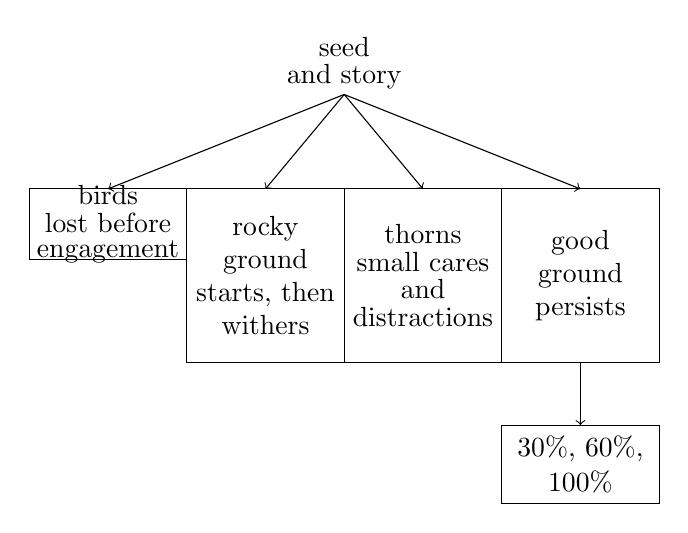
\begin{tikzpicture}[x=1cm,y=1cm]
\node at (0,5.8) {\shortstack{seed\\and story}};
\draw[->] (0,5.4) -- (-3.0,4.2);
\draw[->] (0,5.4) -- (-1.0,4.2);
\draw[->] (0,5.4) -- (1.0,4.2);
\draw[->] (0,5.4) -- (3.0,4.2);

\draw (-4.0,3.3) rectangle (-2.0,4.2);
\node at (-3.0,3.75) {\shortstack{birds\\lost before\\engagement}};

\draw (-2.0,2.0) rectangle (0.0,4.2);
\node at (-1.0,3.1) {\shortstack{rocky\\ground\\starts, then\\withers}};

\draw (0.0,2.0) rectangle (2.0,4.2);
\node at (1.0,3.1) {\shortstack{thorns\\small cares\\and\\distractions}};

\draw (2.0,2.0) rectangle (4.0,4.2);
\node at (3.0,3.1) {\shortstack{good\\ground\\persists}};

\draw[->] (3.0,2.0) -- (3.0,1.2);
\draw (2.0,0.2) rectangle (4.0,1.2);
\node at (3.0,0.7) {\shortstack{$30\%$, $60\%$,\\$100\%$}};
\end{tikzpicture}
\end{figure}

Some seed is lost to birds. In the lecture this means the prospect never even arrives at the meeting. Some seed falls on rocky ground. Here the prospect begins, shows signs of life, and disappears at the first heat. Some seed falls among thorns. Here the life is choked by trivial distractions, little cares, and household debris that somehow outrank a larger opportunity.

The key theoretical move is that these are not interpreted as unique mysteries. They are categories. Rohn repeatedly refuses the question, ``Why exactly this case?'' He does not deny curiosity; he disciplines it. We are not to chase birds, not to register for the ``why'' class, and not to turn ordinary disappointment into a consuming research project.

That is why the operative update rule of this section is not emotional but procedural:
\begin{equation}
\text{sow}
\longrightarrow
\text{loss}
\longrightarrow
\text{discipline disappointment}
\longrightarrow
\text{sow again}.
\end{equation}
The insistence on disciplining disappointment is one of the most exact lines in the lecture. If we do not control the emotional meaning of the early losses, we will leave the field before the good ground appears.

\subsection{Question \& Answer}

\paragraph{Question.} What should we do when people disappear, get talked out of it, or are choked by small distractions?

\paragraph{Answer.} The lecture's answer is surprisingly strict. We do not chase every disappearance, we do not demand a secret cause behind every loss, and we do not stop sowing. We classify the event, accept it as part of the structure, discipline disappointment, and continue.

The good news comes at the end of the story. Good ground exists, and if the sowing continues it will be found. Even then the outputs are not uniform:
\begin{equation}
Y \in \{30\%,60\%,100\%\}.
\end{equation}
Good ground itself splits into levels. Here again Rohn resists endless inquiry. Why are some thirty, some sixty, and some a hundred? That is another class he declines to study in depth. The practical lesson is narrower: let the thirties do thirty, the sixties do sixty, and the hundreds do a hundred. Do not kill yourself trying to turn every thirty into a hundred.

\section{Skills, Recruiting, and Service to the Many}

Only after the philosophy of persistence is in place does the lecture turn to skills. This order matters. Skills are not magic wands; they are the instruments with which the earlier philosophy becomes effective.

The first skill is sales, or in his softer language, sharing. It is not presented as heavy technical mastery but as competent representation of a product one has come to value. The numeric claim is clear:
\begin{equation}
I_{\text{after sales}} \approx 5\,I_{\text{before sales}}.
\end{equation}
He says sales multiplied his income by five. The exact base is modest, but the multiplier is important. A new skill changes scale.

The next skill is recruiting, and here the lecture becomes more architectural. A sponsor is not merely a persuader. A sponsor is a bridge. He helps a person move from darkness to light, from skepticism to faith, from not knowing to knowing, from low confidence to growing confidence. The bridge image matters because it turns recruiting into stewardship rather than pressure.

Organizing comes next: getting people to work together. Promotion follows: inventing smaller recognitions and manageable steps rather than waiting only for major company-level ceremonies. Communication follows: conducting a meeting, using language with care, and above all doing it again after the first miserable attempt. Training and teaching then extend the sequence. Training is how the business works; teaching is how life works. Finally inspiration becomes the culminating skill: helping people see themselves first as they are, and then better than they are.

The lecture then widens again. Greatness is linked to service. Rohn draws this line through the Bible, through John Kennedy, and through Zig Ziglar:
\begin{equation}
\text{service to many} \longrightarrow \text{greatness}.
\end{equation}
The Ziglar formula is even more explicit:
\begin{equation}
\text{help enough people get what they want}
\Longrightarrow
\text{you can have what you want}.
\end{equation}
This is still not formal social science, but the scaling logic is unmistakable. The business gives one a way to affect dozens, hundreds, or thousands of lives, directly and indirectly, and compensation is said to grow accordingly.

\subsection{Question \& Answer}

\paragraph{Question.} How does serving more people become a scalable route to wealth and significance?

\paragraph{Answer.} Because the lecture treats recruiting and organizing as multiplicative rather than merely additive. One does not only sell to one more person. One teaches, sponsors, and coordinates people who themselves begin to affect others. That is why the lecture keeps moving from a few, to many, to dozens, hundreds, and thousands. Service scales because influence scales.

\section{Deserve, Attention, Capital, and the Good Life}

The closing movement returns from scale to discipline. Rohn says we must work with the people who deserve it, not merely with the people who need it. He grounds this in the language of planting and harvest. Need alone does not guarantee a crop; planting does. So sponsor attention should follow response:
\begin{align}
\text{you step} &\Rightarrow \text{I step},\\
\text{you respond} &\Rightarrow \text{I respond},\\
\text{you do not step} &\Rightarrow \text{I do not step}.
\end{align}
This is the local update rule of deserve-not-need.

He then gives the attention allocation rule:
\begin{align}
80\% &\text{ of the people do }20\%\text{ of the business},\\
20\% &\text{ justify individual work},\\
80\% &\text{ are handled primarily by group work}.
\end{align}
The point is not contempt for the larger group. The point is that sponsor time is finite and must be structured.

The same realism governs the warning about helping and carrying. One may help a thousand, but one cannot carry three on one's back. The arithmetic is figurative, but the operational meaning is exact: assistance is scalable; total substitution is not.

The lecture then turns once more to capital. Money is explicitly demoted below skill:
\begin{equation}
\text{money without skill} \not\Rightarrow \text{future},
\qquad
\text{skill} \Rightarrow \text{future}.
\end{equation}
This supports the curious late formulation about capitalism:
\begin{equation}
\text{buy}\to\text{sell}
\qquad\text{or}\qquad
\text{sell}\to\text{buy}.
\end{equation}
The wording in the transcript is noisy, but the intended point is clear enough. Entry into enterprise need not wait on large initial capital if ambition, courage, and action are present.

Finally the lecture broadens into the architecture of a good life. Productivity matters. Friends matter. Spiritual practice matters. The refusal to ``miss anything'' matters, because experience nourishes language, imagination, and character. The inner circle matters because it supplies emotional power. All of this is compressed into one last causal line:
\begin{equation}
\text{live well} \Longrightarrow \text{earn well}.
\end{equation}
Rohn does not mean that refinement mechanically prints money. He means that a nourished, disciplined, connected life becomes audible in the voice, visible in the face, and active in the personality. It changes the human instrument with which all the earlier skills are executed.

\section{Summary}

The lecture begins with a farm boy and ends with a theory of human leverage. First comes philosophy: without it, product and technique do not bite. Next comes the economic hierarchy \(P>W\), made practical through the part-time thresholds \(P_{\mathrm{pt}}=W_{\mathrm{ft}}\) and \(P_{\mathrm{pt}}=2W_{\mathrm{ft}}\). Then comes the control split between wind and sail, which leads directly to self-change. From there the law of averages supplies a workable arithmetic for action under uncertainty, and the story of the sower extends that arithmetic into a durable theory of disappointment and persistence. Only then do the concrete skills of sales, recruiting, organizing, promotion, communication, teaching, and inspiration enter. The lecture closes by insisting that scale comes through service, that attention must follow deserving response, and that business success is finally nested inside the larger task of living well.